\subsection{Khái niệm}
\begin{definition}
\textbf{Đạo hàm} của hàm số $f$ tại giá trị $a$, kí hiệu bởi $f'(a)$, là
    \begin{equation}
        f'(a)=\lim_{\Delta x\rightarrow 0}\frac{f(a+\Delta x)-f(a)}{\Delta x}
    \end{equation}
nếu giới hạn này tồn tại.
\end{definition}

Ý nghĩa hình học trực quan của đạo hàm là nó thể hiện độ dốc của đồ thị và tốc độ biến thiên của hàm số. Ta xét độ dốc của các đường cát tuyến đi qua A:\footnote{Ở đây góc $\theta_M$ và $\theta_N$ có giá trị âm.}
\begin{figure}[H]
\centering 
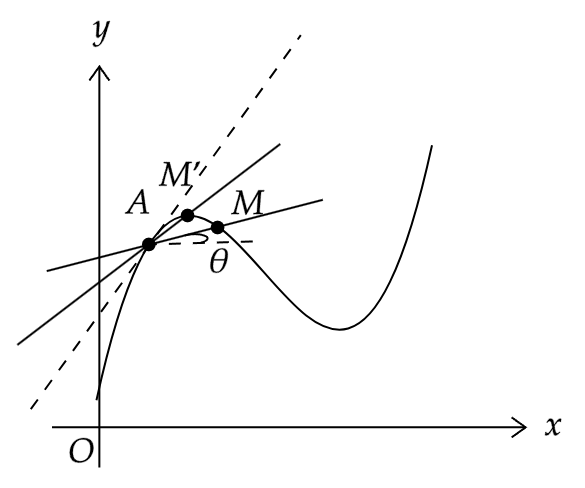
\includegraphics[width=1\textwidth]{Tuan1/ảnh/cattuyen.png}
\caption{Độ dốc của các đường cát tuyến đi qua A (các góc $\theta_M$, $\theta_N$, $\theta_P$)}
\end{figure}

Nếu các điểm $M$, $N$, $P$ tiến gần đến điểm $A$, độ dốc của các đường cát tuyến này sẽ tiến gần đến một giá trị nhất định, chính là độ dốc của tiếp tuyến. Độ dốc này chính là đạo hàm của hàm số tại điểm $A$:
\begin{figure}[H]
\centering
\includegraphics[width=1\textwidth]{Tuan1/ảnh/tocdobienthien.png}
\caption{Liên hệ giữa đạo hàm và độ dốc (độ lớn góc $\theta$) của đồ thị}
\end{figure}

Cũng từ hình vẽ trên, ta có thể thấy đạo hàm chính là hệ số góc của tiếp tuyến đồ thị. Vì thế, ta có thể biểu diễn phương trình của đường tiếp tuyến tại $x=a$:
\begin{equation}
    y=f(a)+f'(a)(x-a)
\end{equation}



\subsection{Một số quy tắc đạo hàm}
Dưới đây là đạo hàm của một số hàm thông dung:

\begin{itemize}
\item\textit{Đạo hàm của hàm đa thức}:
\begin{equation}
    \frac{d}{dx}x^n=nx^{n-1}
\end{equation}
\item\textit{Đạo hàm của các hàm lượng giác}:
\begin{center}
\begin{tabular}{cc}
\(
\begin{aligned}
    &\dfrac{d}{dx}(\sin x)=\cos x\\
    &\dfrac{d}{dx}(\cos x)=-\sin x
\end{aligned}
\)
&
\(
\begin{aligned}
    &\dfrac{d}{dx}(\tan x)=\sec^2 x\\
    &\dfrac{d}{dx}(\cot x)=-\csc^2 x
\end{aligned}
\)
\end{tabular}
\end{center}
\item\textit{Đạo hàm của hàm mũ và hàm logarit}:
\begin{equation}
    \frac{d}{dx}e^x=e^x,\quad \frac{d}{dx}\ln x=\frac{1}{x}
\end{equation}
\end{itemize}

Tương tự như giới hạn, đạo hàm cũng có một số tính chất quan trọng:
\begin{itemize}
    \item \textit{Tính chất tuyến tính}: Nếu $f(x)$ và $g(x)$ là hai hàm số theo $x$, và $c$ là một hằng số, thì
    \begin{equation}
        (cf+g)'=cf'+g'
    \end{equation}
    \item \textit{Quy tắc nhân}: Nếu $f(x)$ và $g(x)$ là hai hàm số theo $x$, thì
    \begin{equation}
        (fg)'=fg'+f'g
    \end{equation}
    \item \textit{Quy tắc chia}: Nếu $f(x)$ và $g(x)$ là hai hàm số theo $x$, với $g(x)\neq 0$, thì
    \begin{equation}
        \left(\frac{f}{g}\right)'=\frac{f'g-fg'}{g^2}
    \end{equation}
\end{itemize}
\subsection{Xấp xỉ tuyến tính và vi phân}
Tiếp theo ta sẽ nói về một ứng dụng quan trọng khác của đạo hàm. Nếu phóng to đồ thị tại điểm $x=a$, ta có thể thấy đồ thị hàm số trông khá gần với tiếp tuyến của nó tại điểm này.
\begin{figure}[H]
\centering
\includegraphics[width=1\textwidth]{Tuan1/ảnh/xapxituyentinh.png}
\caption{Phóng to đồ thị hàm số tại điểm $x=a$}
\end{figure}
Từ quan sát trên, ta có thể nghĩ tới một phép xấp xỉ.

\begin{definition}
    Ở lân cận điểm $x=a$, ta có thể xấp xỉ hàm số $f(x)$ bằng phương trình đường tiếp tuyến tại điểm này:
\begin{equation}
        f(x)\approx f(a)+f'(a)(x-a)
    \end{equation}
đây được gọi là \textbf{xấp xỉ tuyến tính}.
\end{definition}
Ý tưởng đằng sau phép xấp xỉ tuyến tính đôi khi được phát biểu bằng \textbf{phép lấy vi phân}.

\begin{definition}
    Nếu $y=f(x)$, \textbf{vi phân} $dx$ là một biến độc lập. Lúc đó \textbf{vi phân} $dy$ được xác định theo $dx$ bởi phương trình:
\begin{equation}
    dy=f'(x)dx
\end{equation}
\end{definition}
và \textbf{phép lấy vi phân} trên có ý nghĩa hình học như hình vẽ:

\begin{figure}[H]
\centering
\includegraphics[width=1\textwidth]{Tuan1/ảnh/viphan.png}
\caption{Ý nghĩa hình học của phép lấy vi phân}
\end{figure}
Từ kí hiệu bên trên, ta có thể viết lại đạo hàm theo cách khác:
\begin{equation}
    f'(x)=\frac{dy}{dx} 
\end{equation}
Đây được gọi là \textbf{kí hiệu Leibniz cho đạo hàm}.
\subsection{Quy tắc đạo hàm hợp}

Đối với một hàm số \(f(x)\) có dạng phức tạp theo \(x\), ta có thể viết lại nó dưới dạng hàm hợp \(f(g(x))\) sao cho \(f(g)\) và \(g(x)\) có dạng đơn giản hơn, sau đó áp dụng quy tắc sau để thực hiện phép đạo hàm:
\begin{theorem}
\textbf{Quy tắc đạo hàm hợp}: Nếu \(f\) là hàm số có đạo hàm tại \(g(x)\), và \(g\) là hàm số có đạo hàm tại \(x\), thì đạo hàm của hàm hợp \(f(g(x))\) được tính theo công thức:
\begin{equation}
    f'(x)=\frac{df}{dx}=\frac{df}{dg}\cdot\frac{dg}{dx}=f'(g(x))\cdot g'(x)
\end{equation}
\end{theorem}
\textit{Ví dụ: \(f(x)=\sqrt{x^2+1}\) có thể được viết lại dưới dạng hàm hợp \(f(g(x))\) với \(g(x)=x^2+1\).}

\textbf{Lưu ý:} Quy tắc đạo hàm hợp không đơn giản chỉ là khử đi tử và mẫu số giống như phép nhân phân số vì ý nghĩa của kí hiệu Leibniz không hoàn toàn giống với phân số thông thường. Việc chứng minh quy tắc này sẽ phức tạp hơn và sẽ là nhiệm vụ của bạn trong bài tập ....

\subsection{Về tính toán số}
Giả sử ta muốn tính đạo hàm của \(y(x)\) bằng các công cụ lập trình, sẽ là tự nhiên nếu sử dụng trục tiếp định nghĩa của đạo hàm:
\[y(x_0+\epsilon)\approx y(x_0)+\epsilon y'(x_0).\] Ở đây \(\epsilon\) là một con số rất nhỏ, ví dụ như \(0.01\), hay nếu cần chính xác hơn, có thể là \(0.001\),v.v. Như vậy, việc ta cần làm chỉ là khai báo hàm \(y(x)\) rồi chọn một bước nhảy thích hợp. Ta có thể làm điều tương tự đối với các đạo hàm cấp cao hơn: \[y'(x_0 +\epsilon)\approx y'(x_0)+\epsilon y''(x_0).\]
